\chapter{Evaluation of the need}

\section{Helmet HC1 needs}
\begin{wrapfigure}[13]{r}{6cm}
 \begin{center}
	 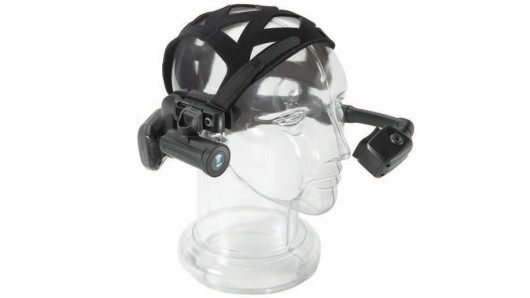
\includegraphics[width=6cm]{images_not_compressed/motorola_hc1.jpg}
		\caption{Picture of the HC1 helmet with the camera plugged}
		\label{hc1}
	 \end{center}
 \end{wrapfigure}

 \par The HC1 Helmet from Motorola is a professional use helmet dedicated to wide or site conditions. It costs around 3000\$ with the camera. It is used to show images in augmented reality in the little screen in front of the left eye. Full voice commanded, it uses an embedded version of windows which was a real problem. You can look at the figure~\ref{hc1} to have an idea of what it looks like.
 
 \par Despite the fact that the Helmet is thought to add functionality, a client of the MIVIA Lab asked them if it was possible to install Linux or Android on the helmet. Even if they lose the voice command system and the drivers to run the camera, etc. They asked me to try, at least, to do it.

\section{The software needs}
 \par At work, when people have to make maintenance of the material, they encounter a problem with the density of the maintenance manuals which can make around 700 pages. We try to ease the maintenance by recreating manuals that focuses on the material that the technician is looking at. To obtain this result, we have to analyze the images of the camera and extract the type of material. That is what the laboratory asked me to do.
 \par This solution can apply to a lot of other objects to find monuments and extract their description for example. To do that I had to use OpenCV pattern detection via SIFT points matching.  
	